\documentclass{standalone}
\usepackage{tikz}
 \usetikzlibrary{decorations.text}

\begin{document}

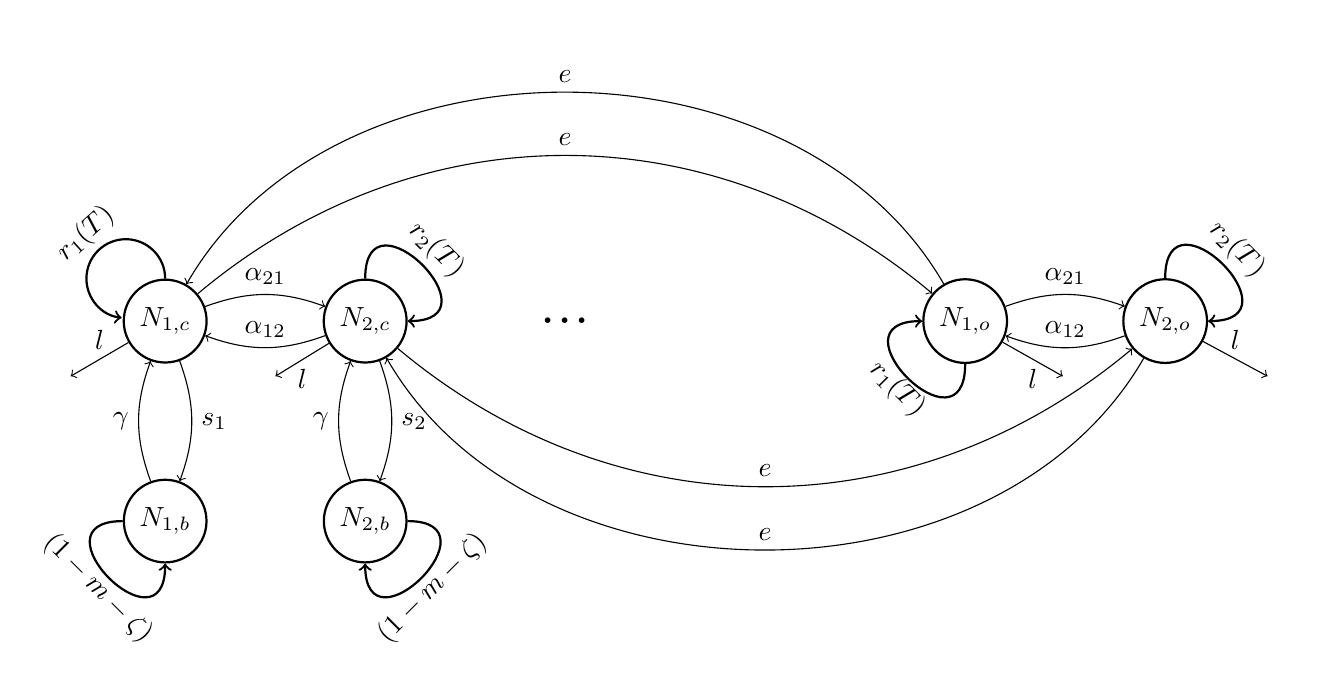
\begin{tikzpicture}
%\tikzstyle{place}=[circle,thick,draw=blue!75,fill=blue!20,minimum size=6mm]
\tikzstyle{place}=[circle,thick,draw=black,fill=white,minimum size=6mm]
\tikzstyle{place}=[circle,thick,draw=black,fill=white,minimum size=6mm]

\begin{scope}
    % Populations
    \node [place](sp1_v){$N_{1,c}$};
    \node [place,node distance=1in,below of=sp1_v](sp1_r){$N_{1,b}$};
    \node [place,right of=sp1_v,node distance=1in](sp2_v){$N_{2,c}$};
    \node [place,node distance=1in,below of=sp2_v](sp2_r){$N_{2,b}$};
    \node [place,right of=sp1_v,node distance=4in](sp1_sea){$N_{1,o}$};
    \node [place,right of=sp1_sea,node distance=1in](sp2_sea){$N_{2,o}$};
   \node [circle,draw=white,fill=white,minimum size=6mm,right of=sp2_v,node distance=1in](sp_etc){\Huge ...}; %all other species

    %Interactions
               \path[->]          (sp2_v)  edge   [bend left=20]   node [above] {$\alpha_{12}$} (sp1_v);
       \path[->]          (sp1_v)  edge   [bend left=20]   node [above] {$\alpha_{21}$} (sp2_v);
       
               \path[->]          (sp2_sea)  edge   [bend left=20]   node [above] {$\alpha_{12}$} (sp1_sea);
       \path[->]          (sp1_sea)  edge   [bend left=20]   node [above] {$\alpha_{21}$} (sp2_sea);
 

     %Growth rates
      \draw[black,thick,->,postaction={decorate,decoration={text along path,raise=5pt,text={{$r_{1}(T)$}{}},text align=center, reverse path}}] (sp1_v.90) arc (-0:264:5mm);
  \draw[thick,->,postaction={decorate,decoration={text along path, raise=5pt,text={{$r_{2}(T)$}{}},text align=center}}] (sp2_v) to [looseness=4, out=90,in=0] (sp2_v);
     \draw[thick,->,postaction={decorate,decoration={text along path, raise=5pt,text={{$r_{2}(T)$}{}},text align=center}}] (sp2_sea) to [looseness=4, out=90,in=0] (sp2_sea);
          \draw[thick,->,postaction={decorate,decoration={text along path, raise=-8pt,text={{$r_{1}(T)$}{}},text align=center,reverse path}}] (sp1_sea) to [looseness=4, out=270,in=180] (sp1_sea);
          
       %cyst mortality   
\draw[thick,->,postaction={decorate,decoration={text along path, raise=-8pt,text={{$(1-m-\zeta)$}{}},text align=center}}] (sp1_r) to [looseness=4, out=180,in=270] (sp1_r);
\draw[thick,->,postaction={decorate,decoration={text along path, raise=-8pt,text={{$(1-m-\zeta)$}{}},text align=center,reverse path}}] (sp2_r) to [looseness=4, out=0,in=270] (sp2_r);
            
       %sinking      
       \path[->]          (sp1_v)  edge   [bend left=20]   node [right] {$s_1$} (sp1_r); 
        \path[->]          (sp2_v)  edge   [bend left=20]   node [right] {$s_2$} (sp2_r);

     %resuspension
       \path[->]          (sp2_r)  edge   [bend left=20]   node [left] {$\gamma$} (sp2_v);
       \path[->]          (sp1_r)  edge   [bend left=20]   node [left] {$\gamma$} (sp1_v);
       
    %exchange
       \path[->]          (sp1_v)  edge   [bend left=40]   node [above] {$e$} (sp1_sea);
                            \path[<-]          (sp1_v)  edge   [bend left=60]   node [above] {$e$} (sp1_sea);
              \path[->]          (sp2_v)  edge   [bend right=40]   node [above] {$e$} (sp2_sea);
                            \path[<-]          (sp2_v)  edge   [bend right=60]   node [above] {$e$} (sp2_sea);
     %vegetative mortality
       \path [->]      (sp1_v)  edge node [above] {$l$}  (-1.2,-0.7); 
       \path [->]      (sp2_v)  edge node [below] {$l$}  (1.4,-0.7); 
       \path [->]      (sp2_sea)  edge node [above] {$l$}  (14,-0.7);                              
       \path [->]      (sp1_sea)  edge node [below] {$l$}  (11.4,-0.7);    
       
       \end{scope}
    
\end{tikzpicture}
\end{document}
